\section{Model cards}
\label{app:modelcards}

\Cref{tab:modelcards} records the six encoders. Each is used through the
Sentence-Transformers interface with mean pooling and $L_2$-normalized output. The two
\mbox{E5} models are queried with the recommended \texttt{query:} prefix for symmetric
similarity; the others take the raw text. Exact weight revisions are pinned in the released
code so that the numbers reproduce against fixed checkpoints. The cross-encoder verifier of
\cref{sec:results} is \texttt{cross-encoder/stsb-roberta-base}, used off the shelf with no
fitting on our pairs.

\begin{table}[t]
  \centering
  \begin{threeparttable}
    \caption{The six audited encoders. Dimensions and parameter counts are the published
      values for each checkpoint.}
    \label{tab:modelcards}
    \begingroup\small
    \begin{tabular}{l r r l l}
      \toprule
      Model & Params (M) & Dim & License & Hugging Face identifier \\
      \midrule
      MiniLM-L6   &  22.7 &  384 & Apache-2.0 & \texttt{sentence-transformers/all-MiniLM-L6-v2} \\
      MPNet-base  & 109.0 &  768 & Apache-2.0 & \texttt{sentence-transformers/all-mpnet-base-v2} \\
      E5-small    &  33.0 &  384 & MIT        & \texttt{intfloat/e5-small-v2} \\
      E5-large    & 335.0 & 1024 & MIT        & \texttt{intfloat/e5-large-v2} \\
      BGE-base    & 109.0 &  768 & MIT        & \texttt{BAAI/bge-base-en-v1.5} \\
      BGE-large   & 335.0 & 1024 & MIT        & \texttt{BAAI/bge-large-en-v1.5} \\
      \bottomrule
    \end{tabular}
    \endgroup
  \end{threeparttable}
\end{table}

\section{Complete results matrix}
\label{app:fullresults}
\Cref{tab:fullresults} is the full record behind the main-text separability table and the
operating-point figures: for every method and domain it gives both threshold-free metrics with
their bootstrap intervals, the precision attainable at three recall targets, and the coverage
attainable under two false-hit ceilings. The pattern that survives every cut is the adversarial
column, where neural and lexical methods alike sit near the base rate; the precision--recall
curves behind these numbers are plotted in \cref{fig:prcurves}.

% Generated from results/reliability_summary.csv and the per-cell JSON reports by make_tables.py
% Auto-generated by experiments/make_tables.py -- do not edit by hand.
\begin{table*}[t]
  \centering
  \begin{threeparttable}
    \caption{Complete reliability matrix for every method and domain: threshold-free
      separability (\prauc{}, \rocauc{}) with $95\%$ \textsc{bca} bootstrap intervals, the
      precision attainable at three recall targets, and the coverage attainable under two
      false-hit ceilings. This is the full record behind \cref{tab:separability,fig:coverage}.}
    \label{tab:fullresults}
    \footnotesize
    \begin{tabular}{l c c c c c r r}
      \toprule
      & \prauc{} & \rocauc{} & \multicolumn{3}{c}{precision @ recall} & \multicolumn{2}{c}{coverage @ \fhr{} (\%)} \\
      \cmidrule(lr){4-6}\cmidrule(lr){7-8}
      Method & (95\% CI) & (95\% CI) & $0.7$ & $0.8$ & $0.9$ & $\le 1\%$ & $\le 5\%$ \\
      \midrule
      \multicolumn{8}{l}{\textit{Questions (base rate 0.36)}}\\[1pt]
      MiniLM-L6 & 0.76\,(0.72,0.78) & 0.87\,(0.85,0.88) & 0.69 & 0.66 & 0.61 & 0.6 & 0.6 \\
      MPNet-base & 0.78\,(0.75,0.81) & 0.89\,(0.87,0.90) & 0.72 & 0.70 & 0.66 & 0.3 & 0.3 \\
      E5-small & 0.74\,(0.70,0.77) & 0.86\,(0.84,0.87) & 0.67 & 0.64 & 0.60 & 0.1 & 0.9 \\
      E5-large & 0.76\,(0.73,0.79) & 0.87\,(0.85,0.88) & 0.69 & 0.65 & 0.62 & 0.6 & 2.4 \\
      BGE-base & 0.76\,(0.72,0.78) & 0.87\,(0.85,0.88) & 0.70 & 0.66 & 0.61 & 0.6 & 1.9 \\
      BGE-large & 0.78\,(0.75,0.80) & 0.88\,(0.86,0.89) & 0.71 & 0.66 & 0.62 & 0.5 & 2.6 \\
      TF-IDF (lexical) & 0.49\,(0.46,0.53) & 0.70\,(0.68,0.72) & 0.51 & 0.50 & 0.47 & 0.0 & 0.0 \\
      Cross-encoder & 0.76\,(0.72,0.79) & 0.87\,(0.85,0.88) & 0.69 & 0.67 & 0.61 & 0.0 & 3.6 \\
      \addlinespace[3pt]
      \multicolumn{8}{l}{\textit{News (base rate 0.68)}}\\[1pt]
      MiniLM-L6 & 0.86\,(0.84,0.87) & 0.76\,(0.73,0.78) & 0.82 & 0.79 & 0.75 & 1.1 & 7.4 \\
      MPNet-base & 0.87\,(0.85,0.89) & 0.78\,(0.76,0.80) & 0.84 & 0.81 & 0.78 & 0.5 & 7.6 \\
      E5-small & 0.89\,(0.88,0.91) & 0.81\,(0.79,0.83) & 0.86 & 0.82 & 0.78 & 8.1 & 21.7 \\
      E5-large & 0.90\,(0.88,0.91) & 0.82\,(0.80,0.83) & 0.86 & 0.83 & 0.79 & 9.1 & 24.4 \\
      BGE-base & 0.88\,(0.87,0.90) & 0.80\,(0.78,0.82) & 0.85 & 0.83 & 0.79 & 4.4 & 18.6 \\
      BGE-large & 0.89\,(0.88,0.91) & 0.81\,(0.79,0.83) & 0.86 & 0.84 & 0.80 & 5.5 & 19.4 \\
      TF-IDF (lexical) & 0.84\,(0.82,0.85) & 0.71\,(0.69,0.74) & 0.79 & 0.76 & 0.72 & 2.1 & 5.9 \\
      Cross-encoder & 0.92\,(0.91,0.93) & 0.84\,(0.83,0.86) & 0.88 & 0.85 & 0.79 & 14.8 & 35.3 \\
      \addlinespace[3pt]
      \multicolumn{8}{l}{\textit{Adversarial (base rate 0.44)}}\\[1pt]
      MiniLM-L6 & 0.59\,(0.55,0.62) & 0.64\,(0.62,0.66) & 0.51 & 0.48 & 0.45 & 0.1 & 0.1 \\
      MPNet-base & 0.60\,(0.57,0.63) & 0.66\,(0.63,0.68) & 0.52 & 0.49 & 0.47 & 0.5 & 0.9 \\
      E5-small & 0.54\,(0.50,0.57) & 0.59\,(0.57,0.62) & 0.47 & 0.46 & 0.45 & 0.1 & 0.1 \\
      E5-large & 0.62\,(0.58,0.65) & 0.67\,(0.64,0.69) & 0.53 & 0.50 & 0.46 & 0.2 & 0.2 \\
      BGE-base & 0.58\,(0.55,0.61) & 0.63\,(0.61,0.65) & 0.50 & 0.48 & 0.45 & 0.1 & 0.1 \\
      BGE-large & 0.62\,(0.58,0.65) & 0.65\,(0.63,0.68) & 0.51 & 0.49 & 0.46 & 0.3 & 0.3 \\
      TF-IDF (lexical) & 0.66\,(0.62,0.69) & 0.72\,(0.70,0.74) & 0.59 & 0.55 & 0.51 & 0.2 & 0.2 \\
      Cross-encoder & 0.51\,(0.48,0.54) & 0.60\,(0.58,0.63) & 0.50 & 0.48 & 0.47 & 0.2 & 0.2 \\
      \bottomrule
    \end{tabular}
    \begin{tablenotes}[flush]\footnotesize
      \item Precision at a recall target is the cleanliness a cache can hold while still
            reusing that share of genuinely reusable answers; coverage at a false-hit ceiling
            is the share of traffic served while keeping errors under the ceiling. The
            cross-encoder is a verifier (not \textsc{ann}-indexable), shown for reference.
    \end{tablenotes}
  \end{threeparttable}
\end{table*}


\begin{figure}[tbp]
  \centering
  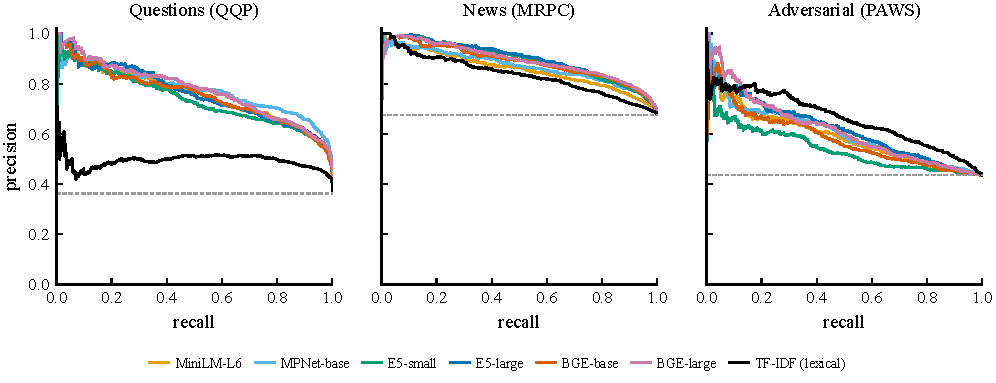
\includegraphics[width=\linewidth]{figures/fig_pr_curves}
  \caption{Precision--recall curves behind the threshold-free separability of
    \cref{tab:separability}. Each curve is one encoder and the dashed line is the domain base
    rate. On the adversarial domain (right) every neural encoder hugs the base rate while the
    lexical control rides above it, the same inversion the main text reports.}
  \Description{Three precision-recall panels, one per domain, each with one curve per encoder
    and a dashed horizontal line at the base rate. On questions and news the neural curves sit
    well above the base rate; on the adversarial domain the neural curves collapse toward the
    base rate while the lexical control curve stays above them.}
  \label{fig:prcurves}
\end{figure}

\begin{figure}[tbp]
  \centering
  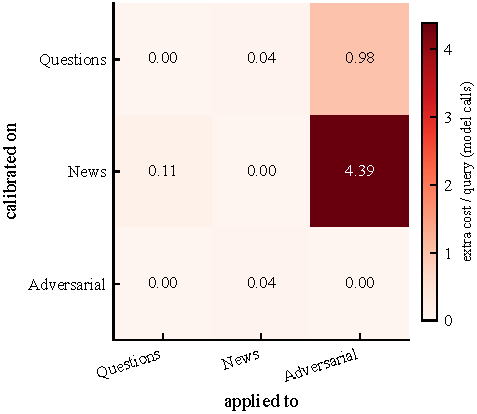
\includegraphics[width=0.62\linewidth]{figures/fig_transfer}
  \caption{\textbf{Thresholds transfer only in the conservative direction} (\cref{sec:calibration}).
    Mean extra cost per query, in model calls, when the cost-aware threshold tuned on one
    domain (row) is applied to another (column), averaged over encoders at $\cfh=20$. A
    threshold tuned on the hard adversarial domain transfers to the easier domains almost for
    free (bottom row); one tuned on an easy domain is too loose for the adversarial one and
    backfires, adding up to $4.4$ model calls per query (right column). The diagonal is
    in-domain, zero by construction.}
  \Description{A three-by-three heatmap with rows labeled by the domain a threshold was
    calibrated on and columns by the domain it was applied to, shaded by the extra cost in
    model calls per query. The diagonal is zero. The cell for a news-calibrated threshold
    applied to the adversarial domain is the darkest at 4.39 and the questions-to-adversarial
    cell is 0.98, while the bottom row of an adversarial-calibrated threshold stays near zero
    across the other domains.}
  \label{fig:transfer}
\end{figure}

\section{Datasheet for the cache-equivalence set}
\label{app:datasheet}

\paragraph{Motivation.}
The set measures whether an embedding cache's similarity decision matches a human notion of
when two prompts may share an answer; the author assembled it for this study.

\paragraph{Composition.}
Each instance is a pair of short English texts with a binary label: cache-equivalent or not.
The pairs are sampled from three public, human-annotated corpora,
\mbox{2500} pairs each: Quora Question Pairs (duplicates)~\cite{wang2019glue}, the
Microsoft Research Paraphrase Corpus (news)~\cite{dolan2005mrpc}, and \mbox{PAWS}
(adversarial word-scrambled paraphrase)~\cite{zhang2019paws}. Base rates of the equivalent
class are $0.36$, $0.68$, and $0.44$ respectively. Exact-duplicate and empty pairs are
removed so that trivial matches do not inflate the positive class.

\paragraph{Collection and labeling.}
Labels are inherited from the source corpora's human annotations; we did not relabel. Sampling
is uniform within each corpus under a fixed seed, preserving the natural base rate. The exact
sampled pairs are released as CSV files.

\paragraph{Uses and limits.}
The set is intended for measuring cache reliability and calibrating thresholds. Its labels
encode paraphrase and duplication, which proxy answer-equivalence imperfectly
(\cref{sec:threats}); it should not be read as a gold standard for answer-equivalence in any
specific application. The source corpora carry their own licenses, which the released code
records; the derived labels and sampling are the author's work.

\section{Reproducibility}
\label{app:repro}

All experiments run on CPU with fixed seeds. The released repository pins dependency versions
and provides the exact commands that regenerate every table and figure from the raw scores. The
whole pipeline, the reliability sweep over seven methods and three domains, the cross-encoder
baseline, and the downstream fault-injection study, runs in well under an hour on a single
modern CPU at zero monetary cost; every model runs locally and no paid \textsc{api} is used. A
single entry point reproduces it end to end: build the labeled set, score it with each method,
compute the bootstrap intervals, run the downstream study, and render the figures.

\section{Pre-specified analysis plan}
\label{app:prereg}

Before the main run we fixed an analysis plan, released with the code, that named the research
questions, the primary metric (\prauc{} under class imbalance, with the false-hit/coverage
frontier as the operating-point view), the encoders and domains, the sample size of
\mbox{2500} pairs per domain, the bootstrap procedure and the multiple-comparison correction,
and the rule that all between-encoder comparison would use threshold-free metrics. This is a
self-recorded plan in the released materials, not a third-party registration. The sample of
\mbox{2500} pairs per domain gives several hundred labeled examples per class in every
encoder--domain cell, which keeps the bootstrap interval on the primary metric narrow,
typically within about $\pm 0.03$ \prauc{} (\cref{tab:separability}). Deviations from the plan,
if any, are reported with their rationale alongside the code.

\section{Claims and evidence}
\label{app:claims}

\Cref{tab:claims} maps each claim this paper makes to the specific table or figure that
supports it, so that a reader can check any one of them directly against the released data.

\begin{table}[t]
  \centering
  \begin{threeparttable}
    \caption{Each headline claim and the evidence behind it.}
    \label{tab:claims}
    \small
    \begin{tabular}{>{\raggedright\arraybackslash}p{0.62\linewidth} l}
      \toprule
      Claim & Evidence \\
      \midrule
      Cache-equivalence is distinct from cosine similarity & \cref{fig:teaser}, \cref{sec:setup} \\
      On adversarial near-duplicates every encoder is near chance (\prauc${}\le 0.62$) & \cref{tab:separability}, \cref{fig:heatmap} \\
      A lexical baseline beats every neural encoder there (paired, $p<0.003$) & \cref{tab:separability}, \cref{sec:results-auc} \\
      A joint cross-encoder verifier also collapses there (\prauc${}=0.51$) & \cref{tab:separability} \\
      Scale barely helps ($+0.08$ \prauc{} from small to large E5) & \cref{tab:separability} \\
      At a $1\%$ false-hit ceiling, coverage is $\approx 9\%$ (news), $<1\%$ (else) & \cref{fig:coverage}, \cref{tab:fullresults} \\
      A false hit costs nearly as much in context as in the answer & \cref{fig:downstream}, \cref{sec:downstream} \\
      A fixed threshold costs several times more than not caching & \cref{tab:calibration} \\
      Cost-aware matches the ceiling policy without a hand-set target & \cref{tab:calibration}, \cref{alg:calib} \\
      A threshold transfers across domains only in the conservative direction & \cref{sec:calibration} \\
      \bottomrule
    \end{tabular}
  \end{threeparttable}
\end{table}

\section{Author contributions}
\label{app:credit}

As the sole author, Sunny Patel is responsible for all roles under the
\textsc{credit} taxonomy: conceptualization, methodology, software, formal analysis,
investigation, data curation, writing (original draft and revision), and visualization.
